%\documentclass[tikz, border=5pt]{standalone}
\begin{document}
	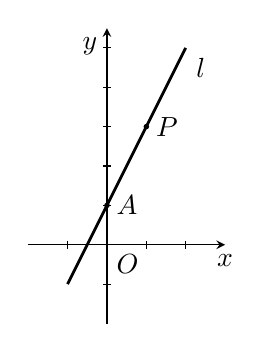
\begin{tikzpicture}[>=stealth, scale=0.5] % 箭头样式为stealth,
		
		% 绘制坐标轴
		\draw[->] (-2,0) -- (3,0) node[below] {$x$}; % x轴(带箭头和标签)
		\draw[->] (0,-2) -- (0,5.5) node[below left] {$y$}; % y轴(带箭头和标签)
		\node at (0,0) [below right] {$O$};           % 原点O的标签
		
		% 绘制所有小刻度线(从 -1 到 2,每隔 1 单位画竖线)
		\foreach \x in {-1,0,...,2} {
			\draw (\x, 0.1) -- (\x, -0.1);  % 小竖线(长 0.2 单位)
		}
		\foreach \y in {-1,0,...,5} {
			\draw (0.1,\y) -- (-0.1,\y);  % 小竖线(长 0.2 单位)
		}
		
		% 定义各关键点坐标
		\coordinate (A) at (0,1);  % 点A
		\coordinate (P) at (1,3); % 点P₂
		
		% 绘制直线l y=2x+1
		\draw[line width=1pt] (-1,-1) -- (2,5) node[below right]{$l$};
		
		% 标记各点的标签
		\fill (A) circle (2pt) node [right] {$A$};  % 带标签的实心点
		\fill (P) circle (2pt) node [right] {$P$};  % 带标签的实心点
		
	\end{tikzpicture}
\end{document}
